% alfak2 sparse joint model, more than two time points: the anchored method
% (series = "anchored", the current default). Mirrors fit_sparse_joint(),
% sparse_joint_uncounted_samples(), sparse_joint_intermediate_dispersion()
% and sparse_joint_used_counts() in R/sparse-joint.R.
% Build: pdflatex flow_anchored.tex
\documentclass[tikz,border=4pt]{standalone}
% Shared style of the alfak2 flowcharts (doc/flowcharts/*.tex).
% Each chart is a standalone document; build one with
%   cd doc/flowcharts && pdflatex <chart>.tex
% or all of them with doc/flowcharts/build.sh. doc/alfak2_method.tex includes
% the PDFs.
\usepackage{amsmath,amssymb}
\usepackage[scaled=0.92]{helvet}
\renewcommand{\familydefault}{\sfdefault}
\usepackage{xcolor}
\usetikzlibrary{positioning,shapes.geometric,shapes.misc,arrows.meta,calc,fit,backgrounds}

% Thresholds of series = "auto" (sparse_joint_auto_thresholds in
% R/sparse-joint-series-methods.R). Change them here when the code changes.
\newcommand{\autoshare}{0.3}
\newcommand{\autoweight}{0.5}

\newcommand{\code}[1]{\texttt{\small #1}}

\definecolor{cIn}{HTML}{DCE6F2}    \definecolor{cInB}{HTML}{4F6D9A}
\definecolor{cProc}{HTML}{F5F5F5}  \definecolor{cProcB}{HTML}{707070}
\definecolor{cDec}{HTML}{FFF2CC}   \definecolor{cDecB}{HTML}{B8902B}
\definecolor{cTwo}{HTML}{D0E4F5}   \definecolor{cTwoB}{HTML}{2E6DA4}
\definecolor{cAnch}{HTML}{D9EAD3}  \definecolor{cAnchB}{HTML}{3D7A33}
\definecolor{cPair}{HTML}{FCE5CD}  \definecolor{cPairB}{HTML}{C0661A}
\definecolor{cState}{HTML}{E6DDF2} \definecolor{cStateB}{HTML}{6A4A9C}
\definecolor{cCore}{HTML}{EFEFEF}  \definecolor{cCoreB}{HTML}{8A8A8A}
\definecolor{cOut}{HTML}{D5EDEA}   \definecolor{cOutB}{HTML}{2C7C73}
\definecolor{cErr}{HTML}{F8D7D7}   \definecolor{cErrB}{HTML}{B03030}
\definecolor{cAuto}{HTML}{FFFBEA}

\tikzset{
  >={Stealth[length=2.4mm,width=1.8mm]},
  every node/.style={font=\small},
  box/.style={draw=#1B, fill=#1, rounded corners=2.5pt, line width=0.7pt, align=left,
              inner xsep=5pt, inner ysep=4pt},
  box/.default=cProc,
  w/.style={text width=#1},
  dec/.style={draw=cDecB, fill=cDec, chamfered rectangle, chamfered rectangle xsep=7pt,
              line width=0.7pt, align=center, inner xsep=3pt, inner ysep=3pt},
  err/.style={box=cErr, font=\footnotesize},
  tag/.style={draw=#1, dashed, rounded corners=6pt, fill=white, font=\scriptsize, inner sep=2.5pt,
              align=center},
  arr/.style={->, line width=0.8pt, draw=black!75},
  darr/.style={->, line width=0.8pt, draw=black!60, dashed},
  lab/.style={font=\footnotesize\itshape, fill=white, inner sep=1.5pt, text=black!85},
  frame/.style={draw=#1, rounded corners=6pt, line width=0.9pt, inner sep=7pt},
  ftitle/.style={font=\footnotesize\bfseries, fill=white, inner sep=2pt, text=#1},
}

\begin{document}
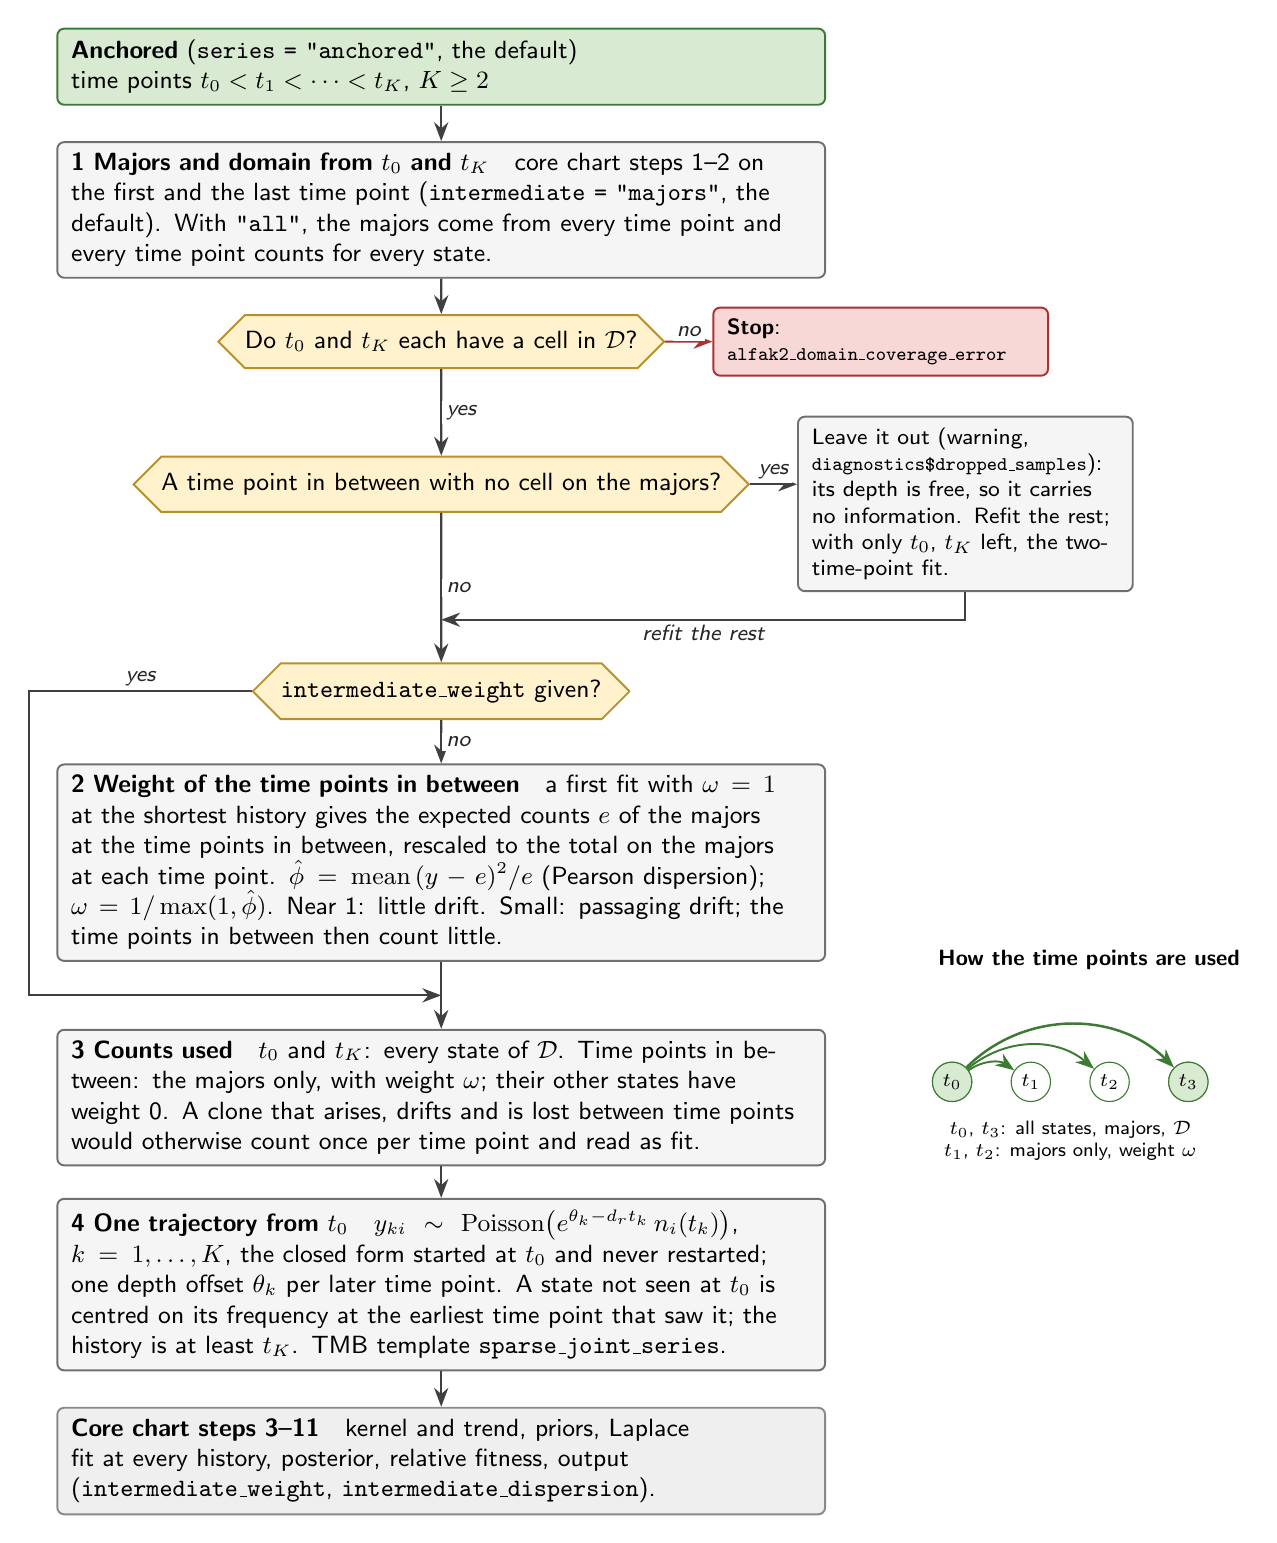
\begin{tikzpicture}

\node[box=cAnch, w=9.4cm] (in) at (0,0) {%
  \textbf{Anchored} (\code{series = "anchored"}, the default)\\
  time points $t_0<t_1<\dots<t_K$, $K\ge2$};

\node[box, w=9.4cm, below=0.45cm of in] (major) {%
  \textbf{1 Majors and domain from $t_0$ and $t_K$}\quad core chart steps 1--2 on the first and the last
  time point (\code{intermediate = "majors"}, the default). With \code{"all"}, the majors come from every
  time point and every time point counts for every state.};
\node[dec, below=0.45cm of major] (cover) {Do $t_0$ and $t_K$ each have a cell in $\mathcal D$?};
\node[err, w=3.9cm, right=0.6cm of cover] (stop) {%
  \textbf{Stop}: {\ttfamily\scriptsize alfak2\_domain\_coverage\_error}};
\draw[arr] (in) -- (major);
\draw[arr] (major) -- (cover);
\draw[arr, draw=cErrB] (cover) -- node[lab, above] {no} (stop);

\node[dec, below=1.1cm of cover] (empty) {A time point in between with no cell on the majors?};
\node[box, w=3.9cm, font=\footnotesize, right=0.6cm of empty, yshift=-0.25cm] (drop) {%
  Leave it out (warning, {\ttfamily\scriptsize diagnostics\$dropped\_samples}): its depth is free, so it carries no
  information. Refit the rest; with only $t_0$, $t_K$ left, the two-time-point fit.};
\draw[arr] (cover) -- node[lab, right] {yes} (empty);
\draw[arr] (empty.east) -- node[lab, above] {yes} (empty.east -| drop.west);

\node[dec, below=1.9cm of empty] (given) {\code{intermediate\_weight} given?};
\draw[arr] (empty) -- node[lab, right] {no} (given);
\draw[arr] (drop.south) |- node[lab, below, pos=0.75] {refit the rest} ($(drop.south -| empty.south)+(0,-0.35)$);

\node[box, w=9.4cm, below=0.55cm of given] (first) {%
  \textbf{2 Weight of the time points in between}\quad a first fit with $\omega=1$ at the shortest history
  gives the expected counts $e$ of the majors at the time points in between, rescaled to the total on
  the majors at each time point. $\hat\phi=\mathrm{mean}\,(y-e)^2/e$ (Pearson dispersion);
  $\omega=1/\max(1,\hat\phi)$. Near 1: little drift. Small: passaging drift; the time points in between
  then count little.};
\draw[arr] (given) -- node[lab, right] {no} (first);

\node[box, w=9.4cm, below=0.85cm of first] (used) {%
  \textbf{3 Counts used}\quad $t_0$ and $t_K$: every state of $\mathcal D$. Time points in between: the
  majors only, with weight $\omega$; their other states have weight 0. A clone that arises, drifts and
  is lost between time points would otherwise count once per time point and read as fit.};
\draw[arr] (first) -- (used);
\draw[arr] (given.west) -- ($(given.west -| first.west)+(-0.35,0)$) node[lab, above, pos=0.5] {yes}
  |- ($(first.south)!0.5!(used.north)$);

\node[box, w=9.4cm, below=0.4cm of used] (model) {%
  \textbf{4 One trajectory from $t_0$}\quad
  $y_{ki}\sim\mathrm{Poisson}\bigl(e^{\theta_k-d_rt_k}\,n_i(t_k)\bigr)$, $k=1,\dots,K$, the closed form
  started at $t_0$ and never restarted; one depth offset $\theta_k$ per later time point. A state not seen
  at $t_0$ is centred on its frequency at the earliest time point that saw it; the history is at least
  $t_K$. TMB template \code{sparse\_joint\_series}.};
\draw[arr] (used) -- (model);

\node[box=cCore, w=9.4cm, below=0.45cm of model] (core) {%
  \textbf{Core chart steps 3--11}\quad kernel and trend, priors, Laplace fit at every history,
  posterior, relative fitness, output (\code{intermediate\_weight}, \code{intermediate\_dispersion}).};
\draw[arr] (model) -- (core);

% ---- schematic --------------------------------------------------------------
\begin{scope}[shift={($(used.east)+(2.6,0.2)$)}]
  \node[font=\footnotesize\bfseries, anchor=west] at (-1.3,1.55) {How the time points are used};
  \foreach \k/\x in {0/-1.0, 1/0.0, 2/1.0, 3/2.0} {
    \node[circle, draw=cAnchB, fill=white, minimum size=5mm, inner sep=0pt, font=\scriptsize] (s\k) at (\x,0) {$t_\k$};
  }
  \node[circle, draw=cAnchB, fill=cAnch, minimum size=5mm, inner sep=0pt, font=\scriptsize] at (s0) {$t_0$};
  \node[circle, draw=cAnchB, fill=cAnch, minimum size=5mm, inner sep=0pt, font=\scriptsize] at (s3) {$t_3$};
  \draw[->, cAnchB, line width=0.7pt] (s0) to[bend left=35] (s1);
  \draw[->, cAnchB, line width=0.7pt] (s0) to[bend left=40] (s2);
  \draw[->, cAnchB, line width=0.9pt] (s0) to[bend left=45] (s3);
  \node[font=\scriptsize, align=center] at (0.5,-0.75) {$t_0$, $t_3$: all states, majors, $\mathcal D$\\
    $t_1$, $t_2$: majors only, weight $\omega$};
\end{scope}

\end{tikzpicture}
\end{document}
